\documentclass[10pt,a4paper]{exam}
\usepackage[utf8]{inputenc}
\usepackage{amsmath}
\usepackage{amsfonts}
\usepackage{bbm}
\usepackage{commath}
\usepackage{amssymb}
\usepackage{booktabs}
\usepackage{blkarray}
\usepackage{systeme}
\usepackage{graphicx}
\usepackage[left=.75in,right=.75in,top=.75in,bottom=.75in]{geometry}

\usepackage{tikz}
\usetikzlibrary{chains}
\printanswers


\author{Ryan Honea}
\title{Time Series Analysis Homework 4}
\begin{document}
\begin{center}
Time Series Homework 5\\
Ryan Honea
\end{center}
\begin{questions}
\question Find Spectral density for the time series below. Also use R to plot those spectral densities where $e_t \sim WN(0,1)$
\begin{parts}
\item $X_t = e_t - \frac{2}{3}e_{t-2}$
\begin{solution}
\begin{align*}
f(\omega) 		&= \frac{\sigma^2}{2\pi}\left| 1 - \frac{2}{3}e^{-2i\omega} \right|^2\\
					&=  \frac{\sigma^2}{2\pi}\left| 1 - \frac{2}{3}\left(\cos(2\omega) - i\sin(2\omega)\right) \right|^2\\
					&=  \frac{\sigma^2}{2\pi}\left( \left(1 - \frac{2}{3}\cos(2\omega)\right)^2 + \left(\frac{2}{3}\sin(2\omega)\right)^2 \right)
\end{align*}
\begin{verbatim}
spectrala <- function(x) {
  cos_part <- (1 - (2/3)*cos(2*x))^2
  sin_part <- ((2/3)*sin(2*x))^2
  full <- cos_part + sin_part
  outer <- (1/(2*pi))
  return(outer*full)
}
\end{verbatim}
\begin{center}
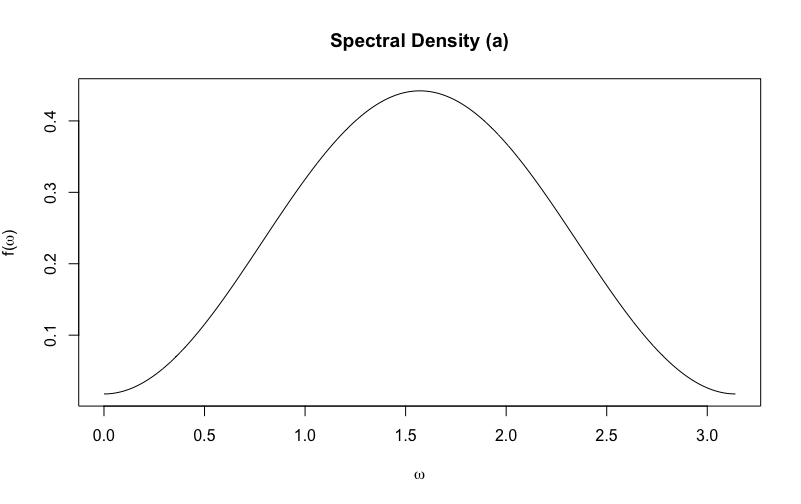
\includegraphics[width = .9\linewidth]{1a}
\end{center}
\end{solution}

\pagebreak

\item $X_t = e_t - \frac{1}{6}e_{t-1} - \frac{1}{6}e_{t-2}$
\begin{solution}
\begin{align*}
f(\omega)		&= \frac{\sigma^2}{2\pi} \left| 1 - \frac{1}{6}e^{-i\omega} - \frac{1}{6}e^{-2i\omega} \right|^2\\
					&=  \frac{\sigma^2}{2\pi} \left| 1 - \frac{1}{6}\left(\cos(\omega) - i\sin(\omega)\right) - \frac{1}{6}\left(\cos(2\omega) - i\sin(2\omega) \right) \right|^2\\
					&=  \frac{\sigma^2}{2\pi} \left| 1 - \frac{1}{6}\left(\cos(\omega) - \cos(2\omega)\right) - \frac{1}{6}i\left(sin(\omega) + \sin(2\omega) \right) \right|\\
					&= \frac{\sigma^2}{2\pi} \left(\left( 1 - \frac{1}{6}\left(\cos(\omega) - \cos(2\omega)\right)\right)^2 + \left(\frac{1}{6}\left(sin(\omega) + \sin(2\omega) \right)\right)^2 \right)
\end{align*}
\begin{verbatim}
spectralb <- function(x) {
  cos_part <- (1 - (1/6)*(cos(x) - cos(2*x)))^2
  sin_part <- ((1/6)*(sin(x) + sin(2*x)))^2
  full <- cos_part + sin_part
  outer <- (1/(2*pi))
  return(outer*full)
}
\end{verbatim}
\begin{center}
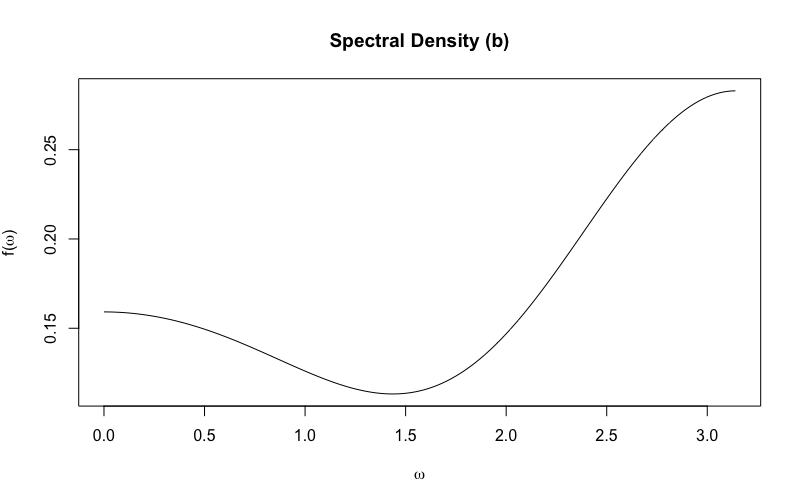
\includegraphics[width = .9\linewidth]{1b}
\end{center}
\end{solution}
\pagebreak



\item $X_t = 0.7X_{t-1} - 0.1X_{t-2} + e_t$
\begin{solution}
\begin{align*}
f(\omega)		&= \frac{\sigma^2}{2\pi} \left| 1 - 0.7e^{-i\omega} - 0.1e^{-2i\omega} \right|^{-2}\\
					&= \frac{\sigma^2}{2\pi} \left| 1 - 0.7\left(\cos(\omega) - i\sin(\omega)\right) - 0.1\left(\cos(2\omega) - i\sin(2\omega)\right)\right|^{-2}\\
					&= \frac{\sigma^2}{2\pi} \left| 1 - 0.7\cos(\omega) - 0.1\cos(2\omega) + i\left(0.7\sin(\omega) + 0.1\sin(2\omega)\right) \right|^{-2}\\
					&= \frac{\sigma^2}{2\pi} \left( \left(1 - 0.7\cos(\omega) - 0.1\cos(2\omega) \right)^2 + \left(0.7\sin(\omega) + 0.1\sin(2\omega) \right)^2 \right)^{-1}
\end{align*}
\begin{verbatim}
spectralc <- function(x) {
  cos_part <- (1 - .7*cos(x) + .1*cos(2*x))^2
  sin_part <- (.7*sin(x) + .1*sin(2*x))^2
  full <- cos_part + sin_part
  outer <- (1/(2*pi))
  return(outer*(full^(-1)))
}
\end{verbatim}
\begin{center}
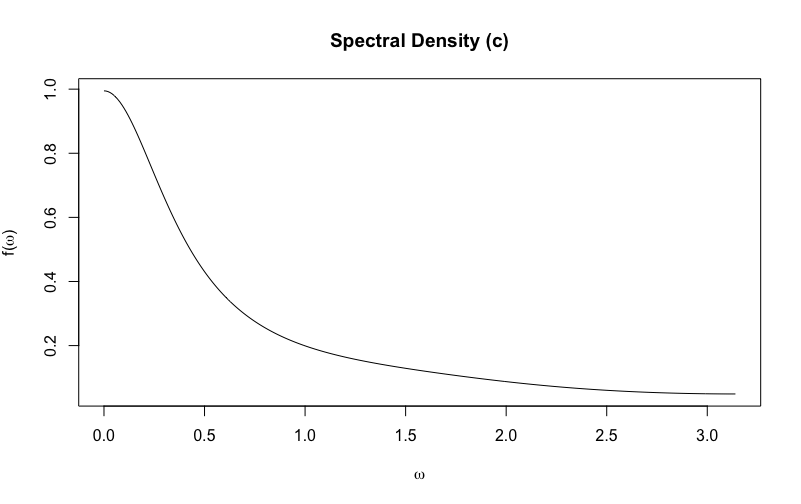
\includegraphics[width = .9\linewidth]{1c}
\end{center}
\end{solution}



\pagebreak
\item $X_t + 0.81X_{t-2} = e_t + \frac{1}{3}e_{t-1}$
\begin{solution}
\begin{align*}
f(\omega) 			&= \frac{\sigma^2}{2\pi}  \left(\frac{\left|1 + \frac{1}{3}\cos(\omega) - \frac{1}{3}i\sin(\omega)\right|^2}{\left|1 + .81\cos(2\omega) - .81i\sin(2\omega)\right|^2}\right)\\
						&= \frac{\sigma^2}{2\pi} \left( \frac{\left(1 + \frac{1}{3}\cos(\omega)\right)^2 + \left(\frac{1}{3}\sin(\omega)\right)^2}{\left(1 + .81\cos(2\omega)\right)^2 + \left(.81\sin(2\omega)\right)^2}				\right)
\end{align*}

\begin{verbatim}
spectrald <- function(x) {
  topcos <- (1 + (1/3)*cos(x))^2
  topsin <- ((1/3)*sin(x))^2
  botcos <- (1 + .81*cos(2*x))^2
  botsin <- (.81*sin(2*x))^2
  full <- (topcos + topsin)/(botcos + botsin)
  outer <- (1/2*pi)
  return(outer*full)
}
\end{verbatim}
\begin{center}
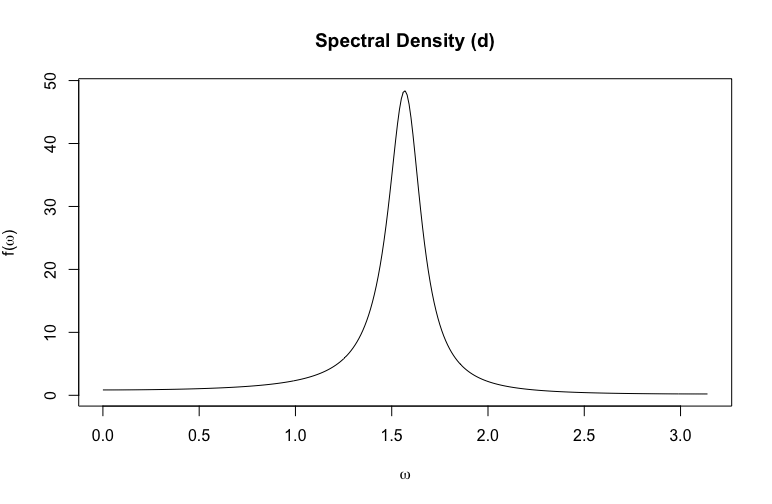
\includegraphics[width = .9\linewidth]{1d}
\end{center}
\end{solution}



\pagebreak
\item $X_t - \frac{3}{4}X_{t-1} + \frac{9}{16}X_{t-2} = e_t + \frac{1}{4}e_{t-1}$
\begin{solution}
\begin{align*}
f(\omega)			&= \frac{\sigma^2}{2\pi} \left( \frac{\left|1 + \frac{1}{4}\cos(\omega) - i\frac{1}{4}\sin(\omega)          \right|^2}{\left|1 - \frac{3}{4}\cos(\omega) + i\frac{3}{4}\sin(\omega)  + \frac{9}{16}\cos(2\omega) - i\frac{9}{16}\sin(2\omega)        \right|^2}    \right)\\
						&= \frac{\sigma^2}{2\pi} \left( \frac{\left(1 + \frac{1}{4}\cos(\omega)\right)^2 + \left(\frac{1}{4}\sin(\omega)\right)^2}{\left(1 - \frac{3}{4}\cos(\omega) + \frac{9}{16}\cos(2\omega)\right)^2 + \left(\frac{9}{16}\sin(2\omega) - \frac{3}{4}\sin(\omega) \right)^2} \right)
\end{align*}

\begin{verbatim}
spectrale <- function(x) {
  topcos <- (1 + (1/4)*cos(x))^2
  topsin <- ((1/4)*sin(x))^2
  botcos <- (1 - (3/4)*cos(x) + (9/16)*cos(2*x))^2
  botsin <- ((9/16)*sin(2*x) - (3/4)*sin(x))^2  
  full <- (topcos + topsin)/(botcos + botsin)
  outer <- (1/2*pi)
  return(outer*full)
}
\end{verbatim}

\begin{center}
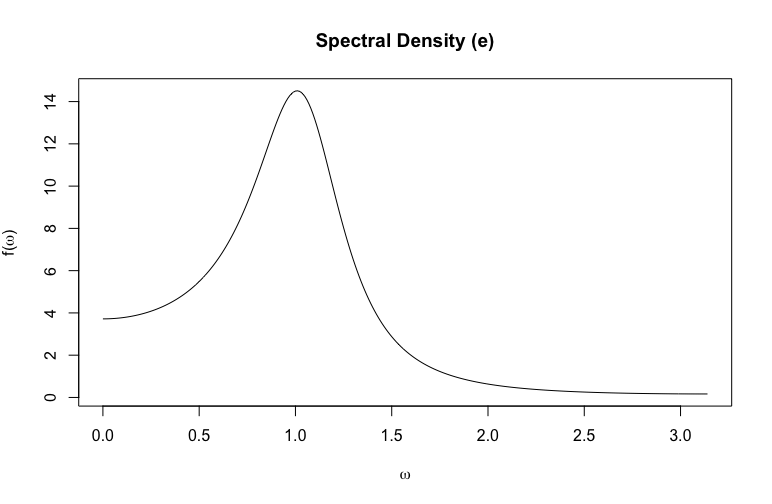
\includegraphics[width = .9\linewidth]{1e}
\end{center}
\end{solution}
\end{parts}

\pagebreak
\question The spectral density of a real-valued time series $X_t$ is defined on $[0,\pi]$ by
\[
	f(\omega) = \begin{cases}
		100,		& \text{for }\frac{\pi}{6}-0.01 < \omega < 
									\frac{\pi}{6} + 0.01\\
		0,	& \text{otherwise} \end{cases}
\]
and on $[\pi, 0]$ by $f(\omega) = f(-\omega)$. Evaluate the ACVF of $\{X_t\}$ at lags 0 and 1.
\end{questions}

\begin{solution}
Utilizing the equation for the autocovariance,
$$\gamma(h) = \int_{-\pi}^{\pi} e^{ih\omega}f(\omega) \dif \omega$$
we can solve this.

\begin{align*}
\gamma(0)			&= \int_{-\pi}^\pi e^{0i\omega} 100 \dif \omega			& \gamma(1)	&= \int_{-\pi}^\pi e^{i\omega} 100 \dif \omega\\
							&= 100\int_{\frac{\pi}{6}-0.01}^{\frac{\pi}{6}+0.01}\dif \omega 	& &= 100\int_{\frac{\pi}{6}-0.01}^{\frac{\pi}{6}+0.01} \cos(\omega) \dif \omega \\
							&= 100 \left(\frac{\pi}{6} + 0.01 - \frac{\pi}{6} + 0.01\right)			& &\approx 100(.0173202)\\
							&= 2				& &\approx 1.73202
\end{align*}
\end{solution}
\end{document}